\documentclass[fontsize=12pt,BCOR=12mm,logo/language=de]{tudcdreprt}
%thpe: BCOR is obviously ignored

%\usepackage[english]{babel}
\usepackage[ngerman]{babel}
\usepackage[babel,german=quotes]{csquotes}
\usepackage[babel]{microtype}
\usepackage{xcolor}
\usepackage{siunitx}
\usepackage{float}
\usepackage[T1]{fontenc}
\usepackage[utf8]{inputenc}

\usepackage{enumerate}
\usepackage{tudcolors}
\usepackage{graphicx}
\usepackage{float}
\usepackage{amsmath}


%thpe: line spacing 1.2-fold (1.2 zeilig) 
\usepackage{setspace}
\setstretch{1.2}

%thpe: Adjust spacing before and after chapter titles to KOMA standards
\RedeclareSectionCommand[
  beforeskip=1cm, % Space before the chapter title
  afterskip=1.5cm % Space after the chapter title
]{chapter}

%thpe: More space for figures and tables
\renewcommand{\floatpagefraction}{0.7}
\renewcommand{\topfraction}{0.8}
\renewcommand{\bottomfraction}{0.5}
\renewcommand{\textfraction}{0.15}


%thpe: Verknüpfung nicht umrandet, Verknüpfung von Tabellen/Grafiken/...
%      Farben noch nicht getestet
\usepackage{hyperref}
%\hypersetup{colorlinks=true, linkcolor=black, citecolor=tudaccent1, menucolor=black, urlcolor=tudaccent5} 

% References and bibliography
\usepackage[style=apa,backend=biber]{biblatex}
\addbibresource{references.bib}

% Title and authors are used in the standard \maketitle command.
% However, it is ignored here as we use a fully user-defined "tudcdtitlepage".
\title{Entwicklung einer Universalmethode zur Umsetzung der Wassserrahmenrichtlinie}

\subtitle{Eine empirische Studie}

\subject{Seminararbeit}

\entity{Institut für Hydrobiologie}

\author{Lisa Wasseramsel}

\date{\today}


\begin{document}

%thpe: suppress page numbering
\pagestyle{empty}

%% --- User-controlled title page ----------------------------------------------
\begin{tudcdtitlepage}

\vspace{-1.8cm}
Fakultät Umweltwissenschaften, Institut für Hydrobiologie, Professur für Limnologie

%\begin{center} % if centered preferred
\setstretch{2.5}
\vspace*{4cm}

\textbf{\huge{Entwicklung einer Universalmethode zur Umsetzung der Wassserrahmenrichtlinie}}

\vspace{1cm}

\textbf{\LARGE{Seminararbeit}}

%\end{center}

%thpe: add flexible space, so that the following block appears at the bottom
%\vspace*{\fill} %does not work in tudcdtitlepage environment

\vspace{6cm} %thpe, todo: make this flexible

\setstretch{1.2}
\begin{tabbing}
	\hspace{0cm} \= \hspace{4cm} \= \kill

	\> Eingereicht von \> Lisa Wasseramsel\\
  \> Matrikelnummer \> 12345678\\
  \> Studiengang \> Bachelor Hydrowissenschaften\\
	\> Erstprüferin \> Prof. Annegret Clearwater (TU Dresden)\\
	\> Zweitprüfer \> Dr. Michael Fischer (Umweltforschungszentrum)\\
	\> Weitere Betreuerin \> M.Sc. Luise Salomon (TU Dresden)\\
	\> Zeitraum \> 03.09.2025 - 23.03.2026\\
	\> Verteidigungsdatum \> 16.04.2026 

\end{tabbing}

\vspace{1cm}

Dresden, \today %thpe: todo use reference to \date

\end{tudcdtitlepage}% ---------------------------------------------------------




\addcontentsline{toc}{chapter}{Zusammenfassung}
\chapter*{Zusammenfassung}

%thpe: page numbering of frontmatter in roman numbers
\pagestyle{plain} % Restore page numbers
\pagenumbering{roman}


Beginne mit einer kurzen Einführung in den Kontext des Themas und stelle die zentrale Aufgaben- bzw. Fragestellung der Arbeit klar.
Beschreibe die angewandte Methodik (z.B. theoretischer Ansatz, empirische Methoden, verwendete Datenbasis).
Präsentiere die wichtigsten methodischen und inhaltlichen Ergebnisse.
Fasse Kernaussagen zusammen und nenne ausgewählte konkrete Befunde.
Schließe mit einem prägnanten Satz, der die Kernbotschaft und ggf. die Bedeutung der Ergebnisse zusammenfasst.

\section*{Abstract}

The abstract should briefly begin by introducing the context of the topic and clearly stating the central research question or objective of the work.
Subsequently, describe the applied methodology (e.g., theoretical approach, empirical methods, data basis used).
Then, present the most important methodological and content-related results, summarizing the key statements and naming selected concrete findings.
Conclude with a concise sentence that encapsulates the core message and, if applicable, the significance of the results.


\tableofcontents

\addcontentsline{toc}{chapter}{Abbildungsverzeichnis}
\listoffigures

\addcontentsline{toc}{chapter}{Tabellenverzeichnis}
\listoftables


% thpe: start new page numbering with page 1 in arabic numbers
\setcounter{page}{1} \pagenumbering{arabic}

\chapter{Einleitung}

Diese Formatvorlage basiert auf der tudscrreprt-Klasse aus dem tudcd-scr-Paket 
\url{https://github.com/tud-cd/tudcd-scr}. Das Paket implementiert das seit 2025 
geltende neue Logo und Corporate Design der TU Dresden und ersetzt die frühere 
tudscrreprt-Klasse von Falk Hanisch.

In der Neuimplementierung sind noch nicht alle Features der vorherigen Version 
implementiert, deshalb musste zum Beispiel die Titelseite mit Standardbefehlen 
zusammengesetzt werden.

Lorem ipsum dolor sit amet, consetetur sadipscing elitr, sed diam nonumy eirmod
tempor invidunt ut labore et dolore magna aliquyam erat, sed diam voluptua. At
vero eos et accusam et justo duo dolores et ea rebum. Stet clita kasd gubergren,
no sea takimata sanctus est Lorem ipsum dolor sit amet. Lorem ipsum dolor sit
amet, consetetur sadipscing elitr, sed diam nonumy eirmod tempor invidunt ut
labore et dolore magna aliquyam erat, sed diam voluptua. At vero eos et accusam
et justo duo dolores et ea rebum. Stet clita kasd gubergren, no sea takimata
sanctus est Lorem ipsum dolor sit amet (siehe Abbildung \ref{fig:fig_1}).

\chapter{Methoden}

Der Methodenteil ist ein zentraler Bestandteil wissenschaftlicher Arbeiten, insbesondere in den Naturwissenschaften. 
Er dient dazu, die angewandten Methoden so darzustellen, dass andere die Ergebnisse reproduzieren können.
Dabei ist es wichtig, die Beschreibung auf das Wesentliche zu beschränken und unnötige Details zu vermeiden.
Untersuchungsobjekte, wie beispielsweise Proben oder Organismen, sollten präzise beschrieben werden, einschließlich ihrer Herkunft, der Bedingungen der Probenentnahme und gegebenenfalls der Lagerung.
Analoges gilt für Datensätze, die man nicht selbst gewonnen hat.
Ebenso müssen die angewandten experimentellen Ansätze, wie Feldarbeit oder Labortechniken, klar skizziert werden.
Methoden, die bereits etabliert sind, müssen nicht vollständig wiedergegeben werden. Stattdessen genügt es, sie kurz in einem bis wenigen Sätzen zu beschreiben und auf die entsprechende Quelle zu verweisen, beispielsweise ein Methodenbuch oder eine Originalpublikation. Wichtig ist jedoch, spezielle Modifikationen klar zu benennen.
Der Schreibstil sollte knapp, präzise und sachlich sein.
Begründungen oder Rechtfertigungen für die Methodenwahl gehören in die Diskussion und sollten im Methodenteil nur ausnahmsweise auftauchen.


\section{Untersuchungsgebiet}

Mit bibLaTeX werden aktive Zitate (auch narrativ genannt) mit \texttt{\textbackslash cite\{\}}: \cite{r-core-2024} und passive Zitate (auch eingeklammert genannt) mit \texttt{\textbackslash parencite\{\}} gesetzt: \parencite{r-core-2024}.

\section{Gewässerbewertung}

\subsection{Vor-Ort-Verfahren}

\subsection{Auswertung von Satellitendaten}

\subsection{Berechnungen}

Mathemathische Gleichungen und Formeln können mit der \texttt{equation} Umgebung gesetzt werden:

\begin{equation}
	y = \alpha + \beta \cdot x + \epsilon
\end{equation}

Für Gleichungen mit mehreren Zeilen eignet sich die \texttt{align} Umgebung gut, bei der man z.B. das Gleichheitszeichen untereinander ausrichten kann.

\begin{align}
\frac{dP}{dt} &= r \cdot f(S) \cdot P \\
\frac{dS}{dt} &= - \frac{1}{Y} \cdot P \\
f(S) &= r_{max} \cdot \frac{S}{k_S + S}
\end{align}

Für Maßeinheiten und chemische Formeln existieren unterschiedliche Methoden. Einfach und pragmatisch ist die Kombination aus Mathematikmodus (mit \verb#$$#) und \verb#mathrm{}#, damit die Maßeinheiten nicht kursiv gesetzt werden.


Code: \verb#$\mathrm{\mu g L^{-1}}$, $\mathrm{PO_4^{3-}}$#

Ergebnis: $\mathrm{\mu g L^{-1}}$, $\mathrm{PO_4^{3-}}$

Das funktioniert soweit, gilt aber typografisch als nicht ganz sauber. Stattdessen werden die Pakete
\textbf{siunitx} und \textbf{mchem} empfohlen.


\section{Statistische Analyse}

Die statistische Analyse wurde mit \textbf{R} \parencite{r-core-2024} und RStudio
\parencite{rstudio-2024} durchgeführt. Für die Grafiken
wurde das Paket \textbf{ggplot2} verwendet \parencite{wickham-ggplot2-2016}.

\section{Test von Umlauten und Sonderzeichen}

Test von Umlauten und Sonderzeichen äöü ÄÖÜ ßßß µ @ €. Dieser Test soll zeigen,
ob die Schriftarten richtig funktionieren, wenn der Text im UTF-8-Format
abgespeichert wurde.



\chapter{Ergebnisse}

Der Ergebnisabschnitt dient der objektiven und neutralen Darstellung deiner Befunde. Konzentriere dich darauf, die Ergebnisse logisch und strukturiert in einer sachlichen Reihenfolge zu präsentieren – ohne sie hier bereits zu interpretieren. Verwende klare und informative Überschriften. Tabellen und Abbildungen (Grafiken, Diagramme, Fotos) müssen selbsterklärend sein. Die Abbildungsunterschrift bzw. Tabellenüberschrift muss fortlaufend nummeriert sein und mit einer aussagekräftigen Beschriftung versehen werden, die nicht zu kurz ist. Als Richtwert gelten zwei bis vier Sätze oder Zeilen, die neben der Beschreibung der Darstellung und der Zuordnung von Farben, Symbolen und Linienarten auch die wichtigste Kernaussage enthalten. Im Text solltest du nur die wichtigsten Befunde zusammenfassen und auf die entsprechenden Abbildungen oder Tabellen verweisen, die die Details zeigen. Stelle dabei die Kernfakten und Hauptergebnisse dar.



\section{Tabellen und Abbildungen}

Tabellen und Abbildungen sind für das Verständnis sehr wichtig. Hierbe sollte ein ausgewogenes verhältnis zwischen Tabellen und Grafiken einerseits und dem erklärenden Text andererseits gewahrt werden. Wichtig ist auch der Lesefluss. Vermeide das zerreißen des Texts durch Abbildungen und Tabelle, bilde stattdessen Textblöcke. Nach einer Überschrift muss immer etwas Text folgen, niemals unmittelbar eine Abbildung oder Tabelle. Da Tabellen und Abbildungen Fließobjekte sind, können sie unter Umständen auch vor der zugehörigen Zwischenüberschrift stehen.

\begin{table}
	\centering
	\caption[Kurzfassung der Tabellenüberschrft]{Langfassung der Tabellenüberschrift,
	        im Regelfall mehrere Zeilen. Es sollten insbesondere Abkürzungen erklärt werden.}
	\label{tab:my_label}
	\begin{tabular}{lll}\hline
		Name & Probenahmestelle & Wert\\\hline
		Temperatur & 1  & 14  \\
		Sauerstof & 2  & 16 \\
		Trübung & 3 & 15 \\ \hline
	\end{tabular}
\end{table}


\section{Weitere Ergebnisse}

Duis autem vel eum iriure dolor in hendrerit in vulputate velit esse molestie consequat, vel illum dolore eu feugiat nulla facilisis at vero eros et accumsan et iusto odio dignissim qui blandit praesent luptatum zzril delenit augue duis dolore te feugait nulla facilisi. Lorem ipsum dolor sit amet, consectetuer adipiscing elit, sed diam nonummy nibh euismod tincidunt ut laoreet dolore magna aliquam erat volutpat.


\begin{figure}
	\centering
	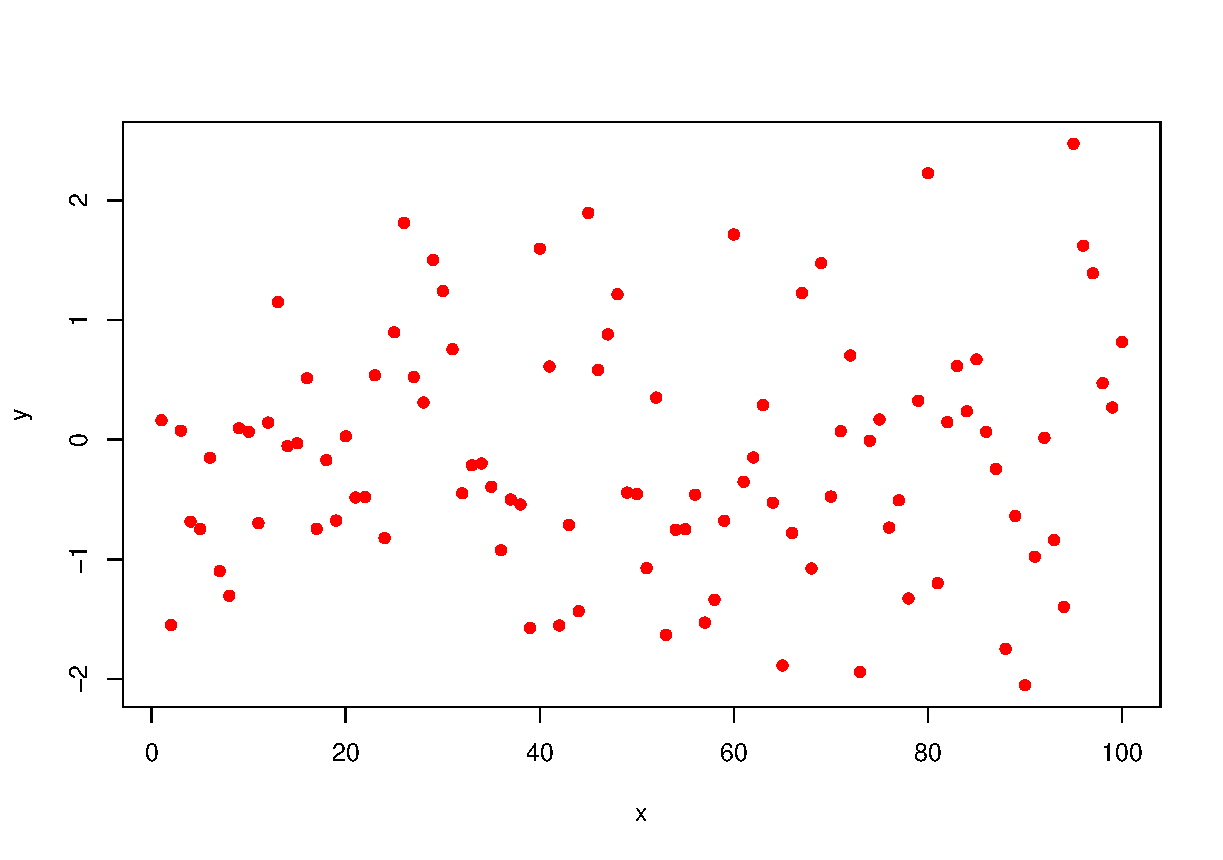
\includegraphics[width=\textwidth]{pdf-plot.pdf}
	\caption[Kurzfassung des Abbildungstitels]{Langfassung des Abbildungstitels,
	         meistens 2-5 Zeilen}\label{fig:fig_1}
\end{figure}

Ut wisi enim ad minim veniam, quis nostrud exerci tation ullamcorper suscipit lobortis nisl ut aliquip ex ea commodo consequat. Duis autem vel eum iriure dolor in hendrerit in vulputate velit esse molestie consequat, vel illum dolore eu feugiat nulla facilisis at vero eros et accumsan et iusto odio dignissim qui blandit praesent luptatum zzril delenit augue duis dolore te feugait nulla facilisi.  

Nam liber tempor cum soluta nobis eleifend option congue nihil imperdiet doming id quod mazim placerat facer possim assum. Lorem


\chapter{Diskussion}

Hier werden die Aufgaben und Hypothesen aus der Einleitung aufgegriffen und
argumentativ untersetzt. Potentielle Defizite und Fehler werden eingeräumt und
eingeordnet. Es sollte das Positive herausgearbeitet werden, außer wenn alles
schief gegangen ist, was selten der Fall ist.

\chapter*{Danksagung} % \chapter*{} erzeugt keine Nummerrierung für das Kapitel und keinen Eintrag im Inhaltsverzeichnis
\addcontentsline{toc}{chapter}{Danksagung} % Ergänzt die Danksagung im Inhaltsverzeichnis


Die Danksagung kann individuell gestaltet werden. Wichtig ist vor allem,
Praxispartnern zu danken und den Leuten oder Organisationen, von denen man
finanziellen Support oder Daten bekommen hat. Bei BMBF-, DFG-, EU- und anderen
Projekten ist die Nennung des Förderkennzeichens in den Förderrichtlinien
vorgeschrieben.

\chapter*{Selbständigkeitserklärung}
\addcontentsline{toc}{chapter}{Selbständigkeitserklärung}

Bei Prüfungs- und Abschlussarbeiten muss eine Selbständigkeitserklärung angegeben werden.
Bitte informiere dich über die gegenwärtig empfohlene Formulierung, z.B.:

Hiermit versichere ich, dass ich die vorliegende Arbeit selbstständig und ohne Benutzung anderer als der angegebenen Hilfsmittel angefertigt habe. Alle Stellen, die anderen Quellen im Wortlaut oder dem Sinn nach entnommen wurden, sind als solche mit Angaben der Herkunft kenntlich gemacht. Dies gilt auch für alle bildlichen Darstellungen. Die Arbeit wurde bisher noch nicht in gleicher oder ähnlicher Form als Prüfungsleistung eingereicht.

Datum, Unterschrift

\paragraph{Erklärung zur Nutzung von KI-Tools:}
Die Verwendung generativer Künstlicher Intelligenz (KI-Tools) zur Optimierung von Formulierungen, zur Fehlerkorrektur oder zur Ideenfindung ist in der Regel nicht verboten, muss aber transparent gemacht werden.

\paragraph{Beispiel:}
Zur Inspiration sowie zur Verbesserung von Formulierungen und der formalen Gestaltung wurde das generative KI-Tool Google Gemini verwendet. Alle wissenschaftlichen Inhalte, Daten und Ergebnisse dieser Arbeit stammen jedoch ausschließlich vom Autor bzw. aus den im Literaturverzeichnis zitierten Quellen. Die inhaltliche Verantwortung liegt vollständig beim Verfasser.

\paragraph{Wichtig:}
KI-Tools dürfen nicht zur selbstständigen Erstellung inhaltlicher Textteile (z.B. der Einleitung, der Diskussion oder der Interpretation von Ergebnissen) verwendet werden, da dies einen Verstoß gegen die Selbständigkeitserklärung darstellt.




\printbibliography


% Falls ein Anhang gewünscht ist kann dieser hier ergänzt werden. Die Kapitel Nummerrierung wird für
% den Anhang auf Buchstaben geändert

\setcounter{chapter}{0}
\renewcommand\thechapter{\Alph{chapter}}
\chapter{Anhang}

Falls ein Anhang nötig ist kann dieser hier ergänzt werden

\begin{figure}[h]
	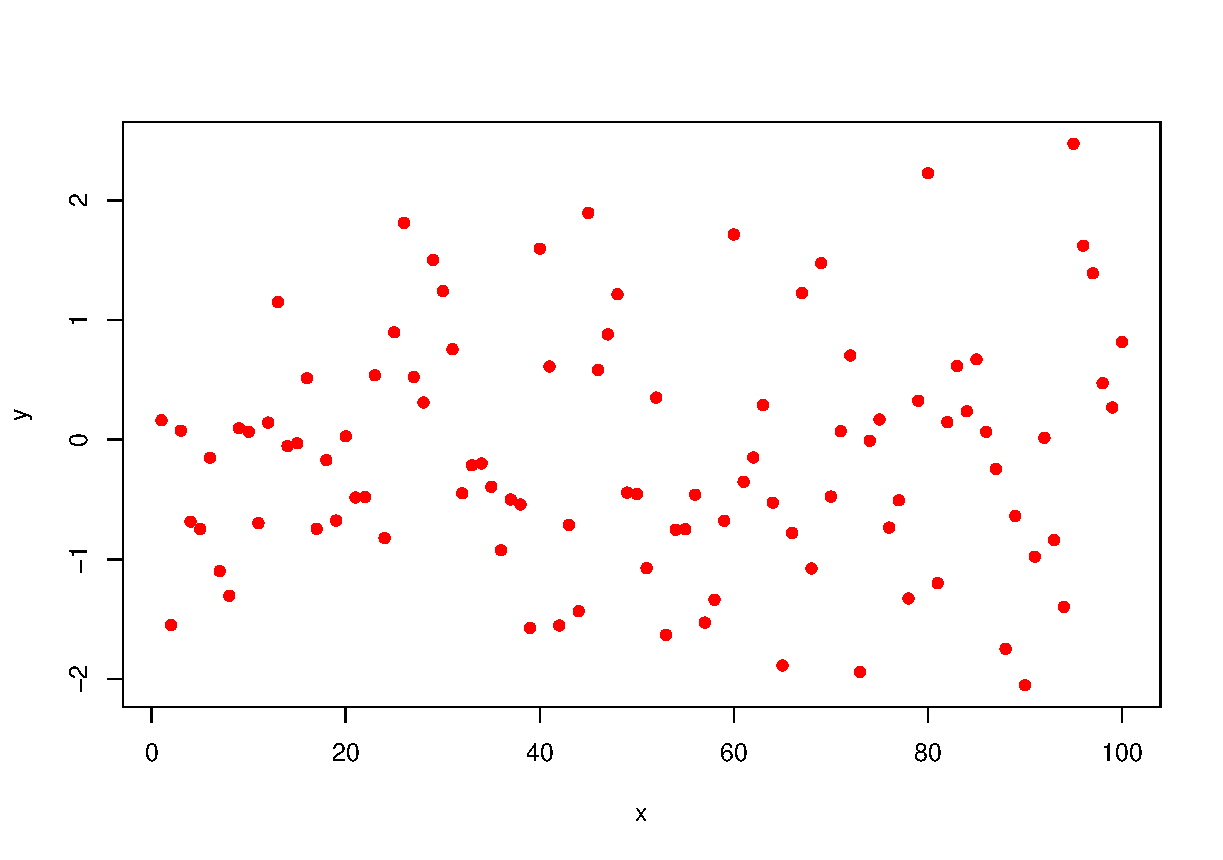
\includegraphics[width=\linewidth]{pdf-plot.pdf}
	\caption[kurze Beschreibung für die Liste der Abbildungen]{Lange Beschreibung für den Fließtext}
\end{figure}



\end{document}
